\important{Update to Judging(August 6th, 2024)}
\chapterauthor{Caleb Bachmeier}
\info{Caleb Bachmeier}{Update to Judging}{August 6, 2024}
\textbf{Goal}: Breakdown Version 1.1 of V5RC High Stake Game Manual
\section*{Update to Judging}
On August 6th 2024, Version 1.0 of the V5RC High Stakes Game Manual was released. This was a pretty minor update, mostly addressing Q\&A's submitted from the V5 community, but the update does change game strategy so this chapter will cover it.
\section*{Definition Updates}
\textbf{Plowing}: The definition of Plowing is has been changed to "\textit{A Robot is considered to be plowing a scoring object if the Robot is intentionally moving it in a preferred direction with a flat or convex face of the Robot or with another Scoring Object.}" Now a robot can't move a Stake with another Stake. Like we saw at the Minnesota Signature Event.
\section*{Rule Changes}
\subsection*{\textless SG5\textgreater}
An addition was made to \textless SG5\textgreater  \textit{"...each preload must be placed such that it is not contacting or encircling a Stake or another scoring objects"}
This is a loophole that was being abused at the Minnesota Signature Event. Teams would place a Ring on a Wall Stake as a preload and hold it up with their robot. This would not score the Ring, therefore before the August 5th Game Manual Update, teams could legally do something shown in \blueref{fig:Preload}{Preload}
\begin{figure}
    \centering
    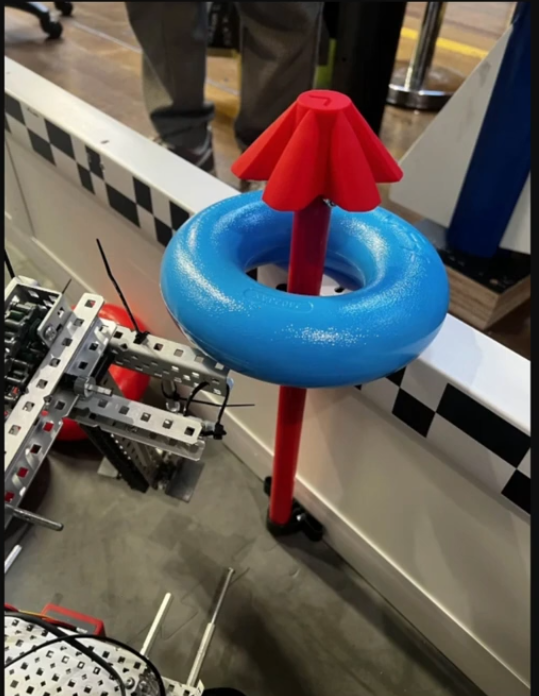
\includegraphics[width=0.5\linewidth]{images/Preload.png}
    \caption{Preload Loophole}
    \label{fig:Preload}
\end{figure}
\subsection*{\textless SG10\textgreater}
An addition was made to \textless SG10\textgreater  clarify that if a Blue Alliance Ring ended up on a Red Alliance Wall Stake it would not count toward anyone's points, but it would count towards the Alliances maximum of two Rings on the Alliance specific Wall Stake.
\section*{Conclusion}
These are all of the updates for this Update to Judging. It was a very minor but useful update, the next major update will be on September 3rd, which will be covered.
\white{September 2024}
\begin{center}
    \begin{tikzpicture}
        % Define the dimensions of the calendar
        \def\year{2024}
        \def\month{9}
        \def\monthname{September}
        \def\startday{1} % 1=Sunday, 2=Monday, ..., 7=Saturday
        \def\numdays{30}
        \def\boxwidth{2} % Width of each box
        \def\boxheight{1.8} % Height of each box

\newcommand{\daytext}[1]{
    \ifcase#1
    \or \cross \or Build Practice  \or Coding Practice \or \cross \or \cross \or Build Practice \or \cross \or \cross \or Build Practice \or Coding Practice
    \or \cross \or \cross \or Build Practice \or  \cross \or \cross \or Build Practice \or Coding Practice \or \cross \or \cross \or Build Practice \or  \cross \or \cross \or Build Practice \or Coding Practice \or \cross \or \cross \or Build Practice \or \cross \or \cross \or Build Practice
    \or Coding Practice
    \fi
}

        % Draw the calendar grid
        \foreach \x in {0, 1, 2, 3, 4, 5, 6, 7} {
            \draw (\x*\boxwidth, 0) -- (\x*\boxwidth, -6*\boxheight);
        }
        \foreach \y in {0, -1, -2, -3, -4, -5, -6} {
            \draw (0, \y*\boxheight) -- (7*\boxwidth, \y*\boxheight);
        }

        % Add day labels
        \node at (0.5*\boxwidth, 0.5*\boxheight) {Sunday};
        \node at (1.5*\boxwidth, 0.5*\boxheight) {Monday};
        \node at (2.5*\boxwidth, 0.5*\boxheight) {Tuesday};
        \node at (3.5*\boxwidth, 0.5*\boxheight) {Wednesday};
        \node at (4.5*\boxwidth, 0.5*\boxheight) {Thursday};
        \node at (5.5*\boxwidth, 0.5*\boxheight) {Friday};
        \node at (6.5*\boxwidth, 0.5*\boxheight) {Saturday};

        % Add the dates in the top left corner and specific text in the middle
        \foreach \d in {1,...,\numdays} {
            \pgfmathtruncatemacro{\col}{mod(\d+\startday-2, 7)}
            \pgfmathtruncatemacro{\row}{-(\d+\startday-2)/7}
            \node[anchor=north west] at (\col*\boxwidth, \row*\boxheight) {\d};
            \node[anchor=center, text width=\boxwidth cm, align=center] at (\col*\boxwidth+0.5*\boxwidth, \row*\boxheight-0.5*\boxheight) {\daytext{\d}};
                                        }

        % Add month and year
        \node at (3.5*\boxwidth, 1.5*\boxheight) {\textbf{\monthname\ \year}};
    \end{tikzpicture}
\end{center}
This is what happened during the month of September. We had full team meetings and build practices every Monday and every Friday, and Ian and Jayden had coding practices every Tuesday. Connor had the robot during this time, Ian has been working on the AI, and Jayden has been working on the simulator, which will have a full chapter on it once in place. At the end of the month we have been driving for quite some time and are ready for tournaments in October.
\begin{comment}
\important{Version 2.0 - September 3, 2024}
\chapterauthor{Caleb Bachmeier}
\textbf{Goal}: Breakdown Version 2.0 of V5RC High Stake Game Manual
\section*{Update to Judging}
On September 3rd, 2024 Version 2.0 of the V5RC High Stakes Game Manual was released. This was a major update to the game manual. This chapter will completely cover the update.

\section*{Rule Changes} 
\end{comment}
\important{Team Meeting (September 5, 2024)}
\chapterauthor{Caleb Bachmeier}
\info{Caleb Bachmeier}{Team Meeting}{September 5, 2024}
\section*{Team Meeting}
We have decided to have a team meeting to talk about roles, future tournaments we would be attending, and our future team branding options. 
\section*{Roles}
We wanted to talk about our different team roles and make sure that the entire team was on the same page. For team roles we wanted to have one "main" team member for the role and one-to-two "backups." These are all listed below:
\subsection*{Practice Roles}
\begin{itemize}
    \item Lead Engineer: Connor, Chase, Ian
    \item Lead Coder: Ian, Jayden
    \item Notebook: Caleb, Ian
    \item Driver: Chase, Miles
    \item Social Media: Miles, Chase
\end{itemize}
The first person in the role is the leader of the role, everyone after the role is the backup, someone that understands the role, and can sufficiently do it if that person is gone.
\subsection*{Tournament Roles}
\begin{itemize}
    \item Drive Team: Chase, Miles, Connor
    \item Scout: Connor
    \item Hypeman: Ian
    \item Pit Crew: Jayden, Caleb
\end{itemize}
\section*{Tournaments}
The current list of tournaments we plan to go to include:
\begin{itemize}
    \item Douglas, South Dakota; October 26th
    \item Grand Forks, North Dakota; November 1st - 2nd
    \item Harrisburg, South Dakota; November 23rd
    \item Mitchell, South Dakota; December 7th 
    \item Groton, South Dakota; Early January 
    \item Rapid City, South Dakota; Early February 
    \item Harrisburg, South Dakota (SD State Event); Late February - Early March
    \item Omaha, Nebraska (CREATE US Open); March 27th - March 29th
    \item Dallas, Texas (High School Worlds); May 6th - May 8th
\end{itemize}
The US Open and Worlds are invitation only, so we hope we'll qualify for those. We wanted to have a team meeting because we wanted to find other tournaments to go to. Our current list of possible events include 
\begin{itemize}
    \item Omaha, Nebraska (Robocalypse); September 28th
    \item Omaha, Nebraska (Tom Dickey Memorial); November 2nd
    \item Omaha, Nebraska (Central High School); November 9th 
    \item Omaha, Nebraska (Antler-Wolf-Storm Classic); November 16th
    \item Omaha, Nebraska (Omaha North High School) December 13th - December 14th
\end{itemize}
Broken down tournament by tournament 
\begin{itemize}
    \item Omaha, Nebraska (Robocalypse); September 28th: \\ We don't believe that Chase and Miles would have enough time to practice driving, so this tournament is out of the question 
    \item Omaha, Nebraska (Tom Dickey Memorial); November 2nd: \\ This tournament only has four teams, so we think this one might be canceled 
    \item Omaha, Nebraska (Central High School); November 9th: \\ Like the previous, this tournament has zero teams, and as the date approaches, this tournament will be canceled 
    \item Omaha, Nebraska (Antler-Wolf-Storm Classic); November 16th: \\ Like the previous two this tournament only has one team registered making it likely for it to be canceled 
    \item Omaha, Nebraska (Omaha North High School) December 13th - December 14th: \\ This tournament only has four teams registered, but we know of multiple teams, such as 7686A, that are planning to register, and this tournament over three months to fill-up, and it's only \$100 to enter. This is the tournament for us
\end{itemize}
Looking at all of these tournaments it seems like the only one that is viable for us is Omaha North High School. We will register and start preparing.
\white{October 2024}
\begin{center}
    \begin{tikzpicture}
        % Define the dimensions of the calendar
        \def\year{2024}
        \def\month{10}
        \def\monthname{October}
        \def\startday{3} % 1=Sunday, 2=Monday, ..., 7=Saturday
        \def\numdays{31}
        \def\boxwidth{2} % Width of each box
        \def\boxheight{1.8} % Height of each box

\newcommand{\daytext}[1]{
    \ifcase#1
     \or Build Practice  \or Coding Practice \or Build Practice \or \cross \or \cross \or \cross \or \cross \or Build Practice \or Coding Practice
    \or Build Practice \or \cross \or \cross \or \cross \or \cross \or Build Practice \or Coding Practice \or Build Practice \or \cross \or \cross \or  \cross \or \cross \or Build Practice \or Coding Practice \or Build Practice \or \cross \or Douglas (No Judging) \or \cross \or \cross \or Build Practice
    \or Coding Practice \or \cross
    \fi
}

        % Draw the calendar grid
        \foreach \x in {0, 1, 2, 3, 4, 5, 6, 7} {
            \draw (\x*\boxwidth, 0) -- (\x*\boxwidth, -6*\boxheight);
        }
        \foreach \y in {0, -1, -2, -3, -4, -5, -6} {
            \draw (0, \y*\boxheight) -- (7*\boxwidth, \y*\boxheight);
        }

        % Add day labels
        \node at (0.5*\boxwidth, 0.5*\boxheight) {Sunday};
        \node at (1.5*\boxwidth, 0.5*\boxheight) {Monday};
        \node at (2.5*\boxwidth, 0.5*\boxheight) {Tuesday};
        \node at (3.5*\boxwidth, 0.5*\boxheight) {Wednesday};
        \node at (4.5*\boxwidth, 0.5*\boxheight) {Thursday};
        \node at (5.5*\boxwidth, 0.5*\boxheight) {Friday};
        \node at (6.5*\boxwidth, 0.5*\boxheight) {Saturday};

        % Add the dates in the top left corner and specific text in the middle
        \foreach \d in {1,...,\numdays} {
            \pgfmathtruncatemacro{\col}{mod(\d+\startday-2, 7)}
            \pgfmathtruncatemacro{\row}{-(\d+\startday-2)/7}
            \node[anchor=north west] at (\col*\boxwidth, \row*\boxheight) {\d};
            \node[anchor=center, text width=\boxwidth cm, align=center] at (\col*\boxwidth+0.5*\boxwidth, \row*\boxheight-0.5*\boxheight) {\daytext{\d}};
                                        }

        % Add month and year
        \node at (3.5*\boxwidth, 1.5*\boxheight) {\textbf{\monthname\ \year}};
    \end{tikzpicture}
\end{center}
This is what happened during the month of October. We had full team meetings and build practices every Tuesday and every Thursday, and Ian and Jayden had coding practices every Tuesday. Ian and Jayden are very close in their respective coding endeavors and will be documenting and implementing in our two planned tournaments on October 26, in Douglas, South Dakota; and on November 1 and 2 in Grand Forks, North Dakota.
\begin{comment}
\important{Autonomaus Planning}
\chapterauthor{Caleb Bachmeier}
\info{Caleb Bachmeier}{}{}
\end{comment}